\documentclass[a4paper,11pt]{article}
\usepackage{a4wide,amsmath,ngerman,url,graphicx}
\usepackage[utf8]{inputenc}
\parskip4pt
\parindent0pt

\newcommand{\br}[1]{\left(#1\right)}
\newcommand{\erf}{\mathrm{erf}}
\newcommand{\m}{\cdot}

\title{Analyse der Coronastatistiken. Teil 2} 
\author{Hans-Gert Gräbe, Leipzig}
\date{Version vom 04.06.2020}

\begin{document}
\maketitle

Dieser Text ist eine Fortschreibung des ersten Teils. Die dortigen
Beschreibungen der allgemeinen Rahmenbedingungen werden als bekannt
vorausgesetzt. 

\section{Logistische Funktion}

Generell ist ein Modell auf der Basis einer \emph{Logistischen Funktion}
\begin{gather*}
  u(t)=\frac{K}{1+C\m\exp(-rt)}\tag{L.1}
\end{gather*}
die anerkanntere Form der Modellierung der Ausbreitung einer Infektion, siehe
dazu den entsprechenden Wikipedia-Eintrag. 
\begin{center}
  \includegraphics[width=.8\textwidth]{LC.png}\\[1em] {Logistische Kurve
    $u(t)=\frac{1}{1+12\exp(-2t)}$ (blau)\\ sowie deren erste (rot) und zweite
    (grün) Ableitung}
\end{center}
$K$ steht dabei für die Sättigungsgrenze $\lim_{t\to\infty}{u(t)}$ und $C$ ist
üblicherweise als $C=\frac{K}{u(0)}-1$ angeschrieben, was sich unmittelbar aus
der Umstellung der Formel für $u(0)$ nach $C$ ergibt. Der Wendepunkt dieser
Funktion und damit das Maximum der ersten Ableitung liegt als Nullstelle der
zweiten Ableitung bei $t_0$ mit $u(t_0)=\frac12\,K$. 

Derartige Funktionen lassen sich deutlich schlechter schätzen als
Glockenkurven, die im Teil 1 dieser Reihe betrachtet wurden und sich durch
Logarithmieren auf einfache Weise auf einen polynomialen Zusammenhang
reduzieren lassen.  Siehe hierzu aber die Arbeit von (Engel 2010) und die
Modellierung mit \textsc{GeoGebra} in (Elschenbroich 2020).

In (Engel 2010) wird insbesondere darauf hingewiesen, dass sich mit einer
guten Schätzung von $K$ die anderen beiden Parameter dann doch mit einem
linearen Fitting bestimmen lassen.  Wir transformieren dazu (L.1) in die
Formel 
\begin{gather*}
  l(t)=\frac{K}{1+\exp(-r(t-m))},\tag{L.2}
\end{gather*}
indem $C=\exp(r m)$ ersetzt wird.  Weiter logarithmieren wir (L.2) und
erhalten als neuen Schätzzusammenhang
\begin{gather*}
  \log\br{\frac{K}{l(t)}-1}=-r(t-m).  \tag{L.3}
\end{gather*}
Der Parameter $K$ ist dabei als Sättigungsgrenze vorab manuell zu schätzen, so
dass die gefittete Kurve möglichst gut auf die Daten passt.  Wir vergleichen
unten diese Ergebnisse mit den Schätzungen auf Basis der Fehlerfunktion aus
Teil 1.

Im Skript ist dazu eine Funktion \texttt{lFit(G,K0)} implementiert, der eine
Liste $G$ von Datenpunkten und der Schätzer für $K$ übergeben werden, wobei in
$G$ zusätzlich vorab alle Datenpunkte mit $y_t\le 10$ ausgefiltert sind.
Weiter wird eine Funktion \texttt{selectData(G,von,bis)} definiert, mit der
aus einer Datenreihe entsprechenden Daten mit $von<t<bis$ selektiert werden
können, um die Modellierungssituation vom 10.04.2020 = Tag 101 nachzustellen.
In einer zweiten Rechnung verwenden wir diese Funktion, um zu sehen, welche
Datenbereiche einer Kurve für eine Schätzung von $l(t)$ besonders gut geeignet
sind.

Wir führen zunächst die Schätzung aus Teil 1 für die Zahl $p(t)$ der positiv
getesteten Personen für die Tage $30\dots 100$ erneut aus (Werte $m_0$, $s_0$
und $K=\sqrt{\pi}\exp(c)\,s$) und verwenden diesen Schätzer für die
Berechnungen einer Parameterschätzung für $l(t)$. Die Schätzungen liegen nahe
beieinander, aber deutlich unter der weiteren Entwicklung der Daten, wie auch
schon aus der Schätzung für die Hubei-Provinz im Teil 1 zu erwarten war.
Siehe dazu die letzte Spalte sowie die beiden Diagramme.
\begin{center}
  \begin{tabular}{|l|c|c|c|c|c|c|}\hline
    Land & $m_0$ & $s_0$ & $K$ & $m$ & $r$ & $p(143)$\\\hline
    Deutschland & 91.83 & 13.40 & 136\,280 & 91.91 & 0.196 & 179\,710\\
    Italien     & 86.68 & 15.38 & 156\,683 & 85.90 & 0.196 & 228\,658\\
    Österreich  & 87.17 & 10.62 &  12\,860 &126.30 & 0.091 &  16\,436\\
    Spanien     & 90.57 & 12.12 & 171\,096 &110.14 & 0.158 & 234\,824\\
  China (Hubei) & 36.52 & 15.95 &  69\,772 & 33.58 & 0.007 &  68\,135\\\hline
  \end{tabular}

  \begin{minipage}{.48\textwidth}\centering
    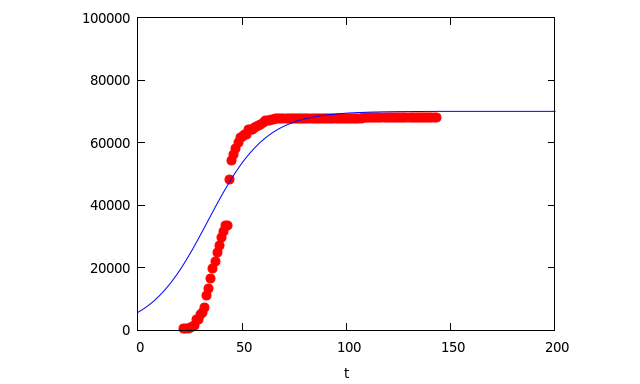
\includegraphics[width=\textwidth]{China-1.png}\\[1em]
                    {Szenario für China (Hubei)}
  \end{minipage}\hfill
  \begin{minipage}{.48\textwidth}\centering
    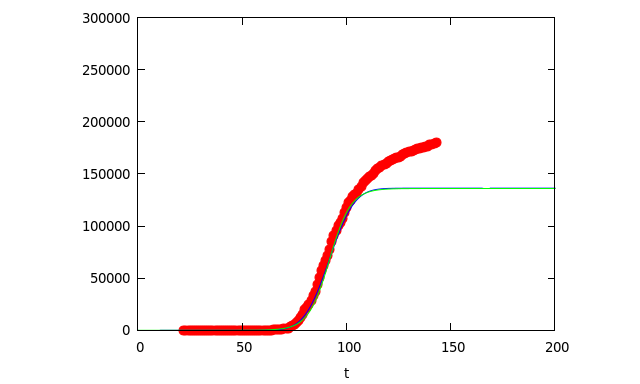
\includegraphics[width=\textwidth]{Germany-1.png}\\[1em]
                    {Szenario für Deutschland}
  \end{minipage}
\end{center}
Neben dem schlechten Schätzer für $K$ sehen wir an den Daten von China mit
deutlich früherem Maximum der Epidemie, dass auch die Wahl des
Schätzintervalls großen Einfluss auf die Güte der Schätzung hat.  Beste
Ergebnisse werden erzielt, wenn Daten aus dem „linearen Teil“ rund um $t=m$
verwendet werden.

Dies ist in der folgenden Übersicht für die logistische Funktion ausgeführt.
Als neuer Schätzer für $K$ wird ein aus $p(143)$ geschätzter Wert verwendet,
als Schätzintervall etwa der Bereich $m-25<t<m+25$. In der folgenden Tabelle
sind Schätzungen aus entsprechenden Zeitreihen der positiv Getesteten für
verschiedene Länder gegenübergestellt, die durch entsprechende
Parameteradjustierungen auf Daten bis zum Tag 143 (22. Mai 2020) gewonnen
wurden:
\begin{center}
  \begin{tabular}{|l|c|c|c|c|c|}\hline
    Land & $K$ & von & bis & $r$ & $m$ \\\hline
    Deutschland & 200\,000 & 70 & 120 & 0.116 & 100.34\\
    Italien & 250\,000 & 70 & 120 & 0.056 & 103.15\\
    Österreich & 18\,000 & 70 & 120 & 0.116 & 95.30 \\
    Spanien & 270\,000 & 70 & 120 & 0.118 & 100.81 \\
    China (Hubei) & 70\,000 & 22 & 62 & 0.213 & 42.51\\
    Schweden & 50\,000 & 100 & 150 & 0.048 & 128.96\\\hline
  \end{tabular}
  \vskip1em

  \begin{minipage}{.3\textwidth}\centering
    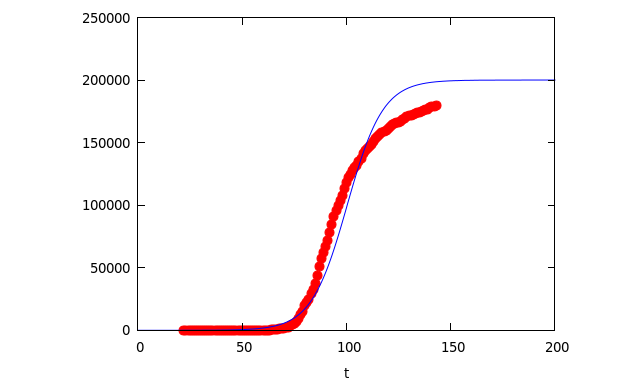
\includegraphics[width=\textwidth]{Germany-2.png}\\[1em] {Deutschland}
  \end{minipage}\hfill
  \begin{minipage}{.3\textwidth}\centering
    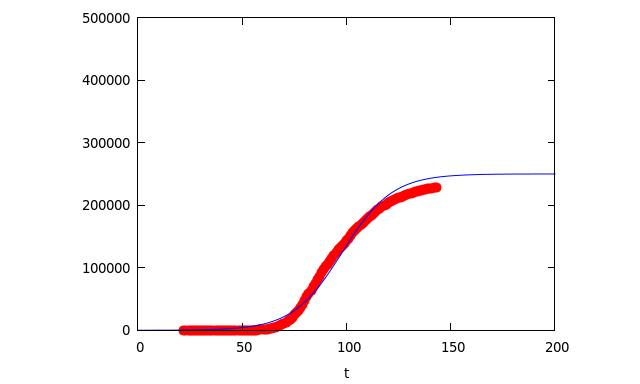
\includegraphics[width=\textwidth]{Italy-2.png}\\[1em] {Italien}
  \end{minipage}\hfill
  \begin{minipage}{.3\textwidth}\centering
    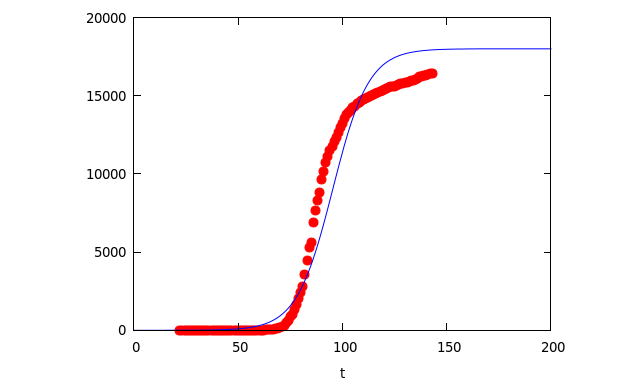
\includegraphics[width=\textwidth]{Austria-2.png}\\[1em] {Österreich}
  \end{minipage}
  
  \begin{minipage}{.3\textwidth}\centering
    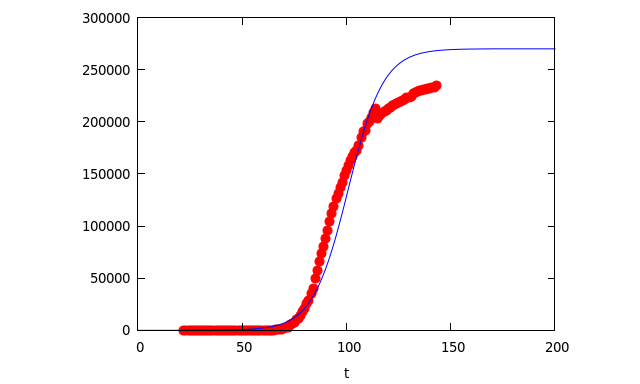
\includegraphics[width=\textwidth]{Spain-2.png}\\[1em] {Spanien}
  \end{minipage}\hfill
  \begin{minipage}{.3\textwidth}\centering
    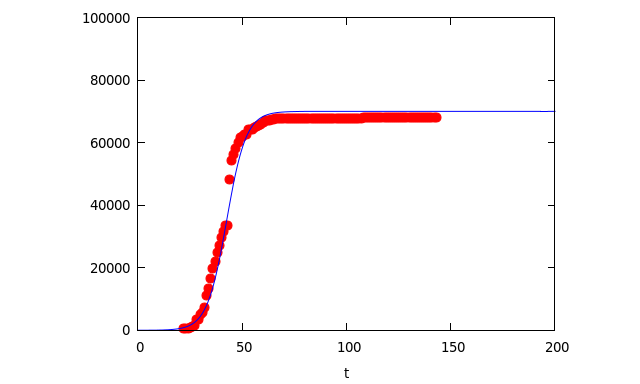
\includegraphics[width=\textwidth]{China-2.png}\\[1em] {China (Hubei)}
  \end{minipage}\hfill
  \begin{minipage}{.3\textwidth}\centering
    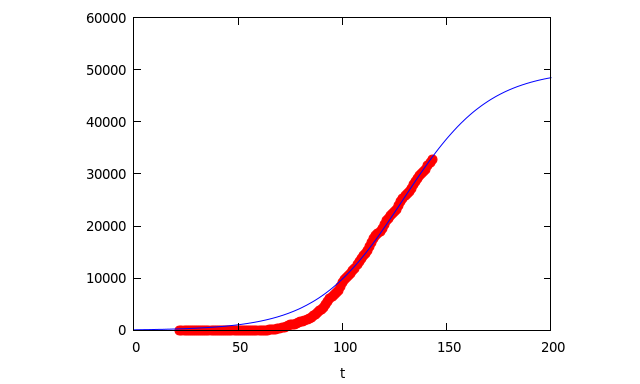
\includegraphics[width=\textwidth]{Sweden-2.png}\\[1em] {Schweden}
  \end{minipage}
\end{center}
In den Diagrammen ist die (etwas zeitversetzte) Abflachung der Kurven nach dem
Lockdown in verschiedenen europäischen Ländern deutlich zu sehen, dessen
Wirkung in das hier verwendete zeithomogene Modell natürlich nicht eingehen
kann.  Dies bleibt gesondert zu untersuchen. 

\section{Literatur}

\begin{itemize}
\item Hans-Jürgen Elschenbroich. Corona: Mathematik \& Modellbildung.\\
  \url{https://www.geogebra.org/m/cfammtpe}.  2020.
\item Joachim Engel. Parameterschätzen in logistischen Wachstumsmodellen.
  Stochastik in der Schule 30 (2010) 1, S. 13–18.
\end{itemize}

\end{document}
